\documentclass{article}
\usepackage[utf8]{inputenc}
\usepackage{graphicx}
\begin{document}

\title{Spikefinder competition\\ convi6: a convolutional network model predicting spikes from calcium signals}
\maketitle
\begin{center}
{\author{Nikolay Chenkov and Thomas McColgan}}
\end{center}

The submitted solution is generated by a convolutional neural network. Here 
we describe some basic properties of the model and discuss possible extensions
and improvements for future algorithms.

\section*{Methods}

The inputs to the network are the calcium signal and an index vector denoting
from which dataset the inputs are from. The network consists of 8 convolutional
layers and one recurrent layer (LSTM). The learning is achieved by downsampling 
the predicted spike rate to 25 Hz and minimizing
the Pearson correlation to the ground-truth spiking
data. The used optimization method is `Adam'.

\begin{figure}
  \centering
  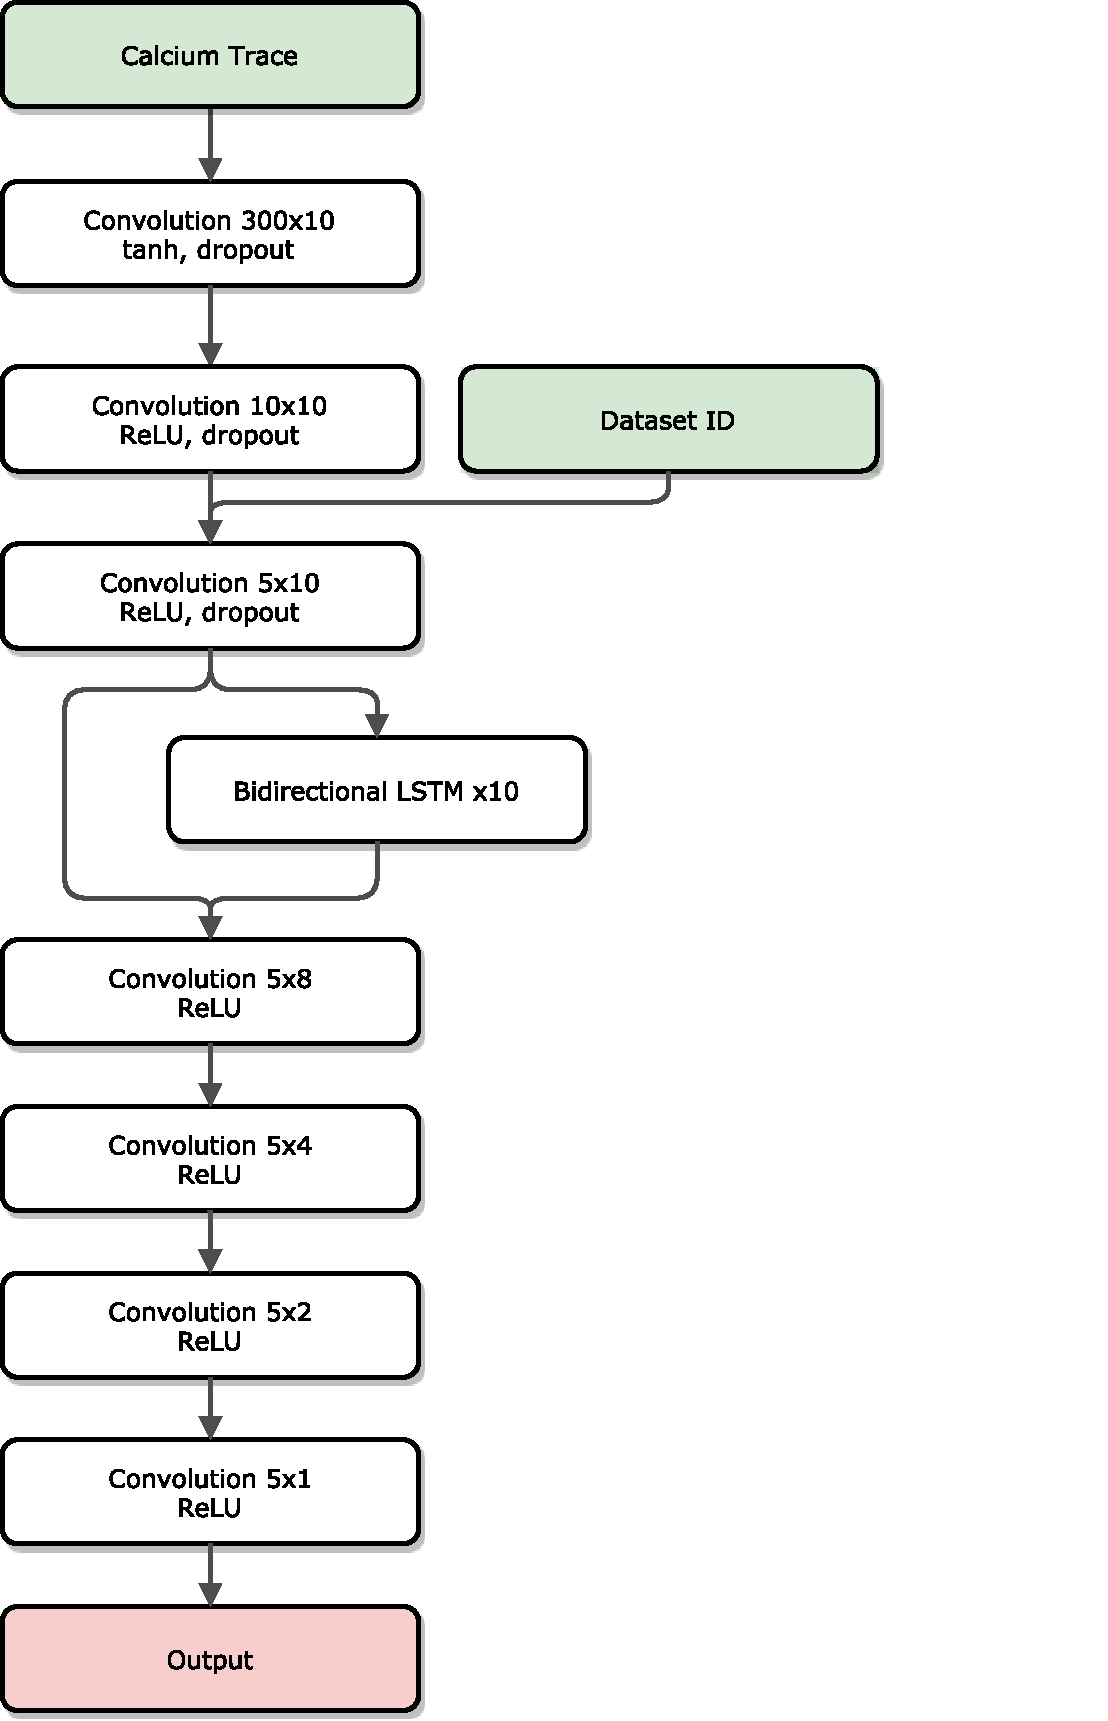
\includegraphics[height=0.9\textheight]{convi}
  \caption{Network Architecture. In the convolutional layers the notion $m$x$n$ denotes $n$ units with
  kernel width of $m$ time steps. }

\end{figure}

The model is depicted in Figure 1.
The first layer consists of 10 units. Each unit uses a kernel with a width of
300 datapoints (3 seconds) that is convolved (actually correlated) with the
input calcium signal. The learned kernels catch a basic repertoire of dynamics
as shown in Figure 2. The output of this layer is passed through a hyperbolic tangent 
activation function (`tanh'). This layer is followed by multiple convolutional layers
with smaller kernel widths (100 and 50 ms, or 10 and 5 time steps, respectively) and with rectified linear activation
functions (`ReLU'). The dataset index is encoded in one-shot fashion, and is
concatenated to the output of the second layer and feed into the input of the third
layer. Moreover, a recurrent neural group (a bidirectional LSTM layer) is fed by the
input of the third layer, and its output is added to the input to the fourth layers.
The following 4 layers have decreasing size, as the last layer consists of a single unit.

\begin{figure}
  \centering
  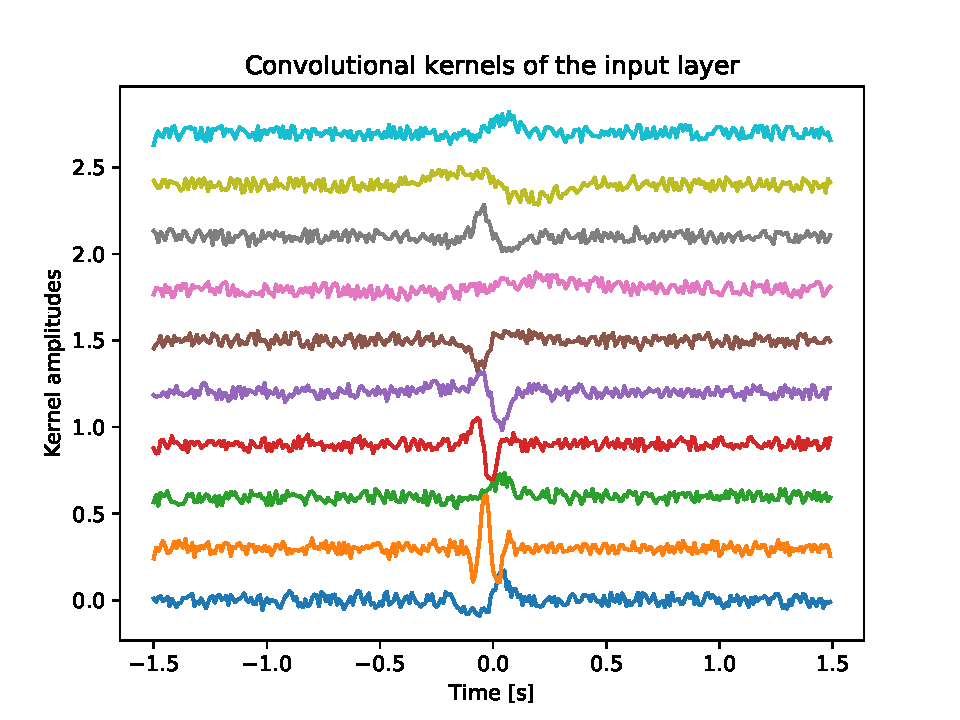
\includegraphics[width=\textwidth]{input_kernels}
  \caption{Example of convolutional kernels learned by the model. The ten kernels of the first convolutional layer (color coded) can describe a wide range of transient calcium dynamics around the time point 0.}
\end{figure}

To distribute the amount of information that different units are caring, a
dropout is applied at the output of the first 5 convolutional layers. An
attempt to apply a batch normalization failed.

The code, including a Docker file, can be found in GitHub:\\ https://github.com/kleskjr/spikefinder-solution

\section*{Discussion}
The model architecture was chosen ad-hoc and is likely to be suboptimal for
the problem it is intended to solve. It could be optimized further by tuning
the network architecture and hyper-parameters by using tools like Spearmint. Moreover, a larger
number of epochs during training might be required. Due to limited computational power we used 50 epochs for
this particular solution.

One observation (to be confirmed) is that plugging the Dataset ID input before the recurrent layer improved the performance of the model. Thus, the dataset information might set different states of the recurrent layer dynamics.

\end{document}

